\documentclass[output=paper,colorlinks, citecolor=brown]{langscibook}
\ChapterDOI{10.5281/zenodo.15006597}
\author{Julian Blaßnigg\affiliation{University of Salzburg} and Irmtraud Kaiser\affiliation{University of Salzburg} and Peter Mauser\affiliation{University of Salzburg} and Konstantin Niehaus\affiliation{University of Salzburg}}
\title{The ``Atlas of colloquial German in Salzburg''}
\subtitle{An update on (areal) variation in a central region of Austria}

\abstract{This article is concerned with the application of geolinguistic methods onto messy big data in dialectology. It presents data from an on-going project, the ``Atlas of Colloquial German in Salzburg'' (\textit{Atlas zur Salzburger Alltagssprache}, ASA), which collected data on language use via a large online survey. The questionnaire consisted of 76 items, each of them given in a situational context. The goal of the project is to provide a first detailed description of the everyday German in the federal state of Salzburg, ranging from local dialect to regional dialect (regiolect) to near-standard and standard. The present study provides first results and identifies areas with similar diatopic variation in Salzburg via a cluster analysis of a total of approx. 10,000 data sets (collected via online questionnaires). Regional Spatial Planning Areas (\textit{Planungsregionen}) prove to be a relevant category in order to account for diatopic variation in the state of Salzburg, with clusters of more traditional, dialect-orientated areas in the south, a regiolectal central area, and a northern urban area (encompassing the capital Salzburg City) orientated towards standard German. The article shows that even with anonymous and uncontrolled data collections, the cluster analysis offers a suitable approach towards larger dialect/regiolect areas as well as smaller transition areas. Ultimately, these methods may prove useful not only for the dialectology of (Austrian) German but also for other languages.
\keywords{german dialects, language variation and change, geolinguistics, German in Austria}}
\IfFileExists{../localcommands.tex}{
  \addbibresource{../localbibliography.bib}
  \usepackage{tabularx,multicol}
%\usepackage{multirow}
\usepackage{subcaption}
\usepackage{url}
\urlstyle{same}

\usepackage{datetime}
\usepackage{enumitem}
\usepackage{langsci-optional}
\usepackage{langsci-lgr}
\usepackage{langsci-branding}

\usepackage{longtable}
\usepackage{xltabular}
\usepackage[linguistics, edges]{forest}
\usepackage{pgfplots}
\pgfplotsset{compat=1.18}
\usetikzlibrary{patterns, tikzmark}
\usepackage{pgfplotstable}
\usepgfplotslibrary{colorbrewer}
\usepackage{listings}
\lstset{basicstyle=\ttfamily,keywordstyle=\normalfont,language=,breaklines=true}

\usepackage{siunitx}
\sisetup{group-digits=none, detect-all=true}

\usepackage{langsci-gb4e}

  \makeatletter
\let\thetitle\@title
\let\theauthor\@author
\makeatother

% Use this Chinese font shipped with TeX Live instead of Source Han, because
% it is more portable/leightweight. Install the "fandol" package from CTAN to
% automatically get this font.
\newfontfamily{\ChineseFandolSong}{FandolSong-Regular.otf}

  %% hyphenation points for line breaks
%% Normally, automatic hyphenation in LaTeX is very good
%% If a word is mis-hyphenated, add it to this file
%%
%% add information to TeX file before \begin{document} with:
%% %% hyphenation points for line breaks
%% Normally, automatic hyphenation in LaTeX is very good
%% If a word is mis-hyphenated, add it to this file
%%
%% add information to TeX file before \begin{document} with:
%% %% hyphenation points for line breaks
%% Normally, automatic hyphenation in LaTeX is very good
%% If a word is mis-hyphenated, add it to this file
%%
%% add information to TeX file before \begin{document} with:
%% \include{localhyphenation}
\hyphenation{
    a-na-ly-sis
    ap-proach-es
    ar-che-o-log-i-cal
    Ar-khan-gelsk
    be-schrei-ben
    Buch-holtz
    Che-lya-binsk
    con-so-nant
    dia-lect
    dia-lect-ology
    Di-a-lekt-for-schung
    Dia-lekt-for-schung
    East-pha-lian
    För-der-ung
    Ge-mein-schaft-lich-keits-ent-wür-fe
    his-tor-i-cal
    Hok-kai-do
    ja-pa-nese
    Ja-pa-nese
    Ka-go-shi-ma
    Ka-li-nin-grad
    Knja-zev
    Ma-kro-be-reich
    Ma-lay-sia
    mor-pho-log-i-cal
    Mos-cow
    Nef-te-yu-gansk
    non-mobile
    nu-cle-ar
    ös-ter-rei-chi-sche
    par-a-digm
    per-zep-ti-ons-lin-gu-is-ti-sche
    plu-ri-zen-tri-schen
    quick-ly
    Reich
    Sax-on
    Schrö-der
    sear-ching
    ste-reo-type
    strength-en-ing
    strong-est
    Stutt-gart
    su-pra-seg-men-tal
    teach-er
    to-po-gra-phy
    To-ron-to
    tra-di-tion-al
    ul-ti-mate-ly
    Um-gangs-spra-che
    Volks-kun-de
    vor-zu-stel-len
    wheth-er
    Wie-sing-er
    with-in
    Wort-at-las
}

\hyphenation{
    a-na-ly-sis
    ap-proach-es
    ar-che-o-log-i-cal
    Ar-khan-gelsk
    be-schrei-ben
    Buch-holtz
    Che-lya-binsk
    con-so-nant
    dia-lect
    dia-lect-ology
    Di-a-lekt-for-schung
    Dia-lekt-for-schung
    East-pha-lian
    För-der-ung
    Ge-mein-schaft-lich-keits-ent-wür-fe
    his-tor-i-cal
    Hok-kai-do
    ja-pa-nese
    Ja-pa-nese
    Ka-go-shi-ma
    Ka-li-nin-grad
    Knja-zev
    Ma-kro-be-reich
    Ma-lay-sia
    mor-pho-log-i-cal
    Mos-cow
    Nef-te-yu-gansk
    non-mobile
    nu-cle-ar
    ös-ter-rei-chi-sche
    par-a-digm
    per-zep-ti-ons-lin-gu-is-ti-sche
    plu-ri-zen-tri-schen
    quick-ly
    Reich
    Sax-on
    Schrö-der
    sear-ching
    ste-reo-type
    strength-en-ing
    strong-est
    Stutt-gart
    su-pra-seg-men-tal
    teach-er
    to-po-gra-phy
    To-ron-to
    tra-di-tion-al
    ul-ti-mate-ly
    Um-gangs-spra-che
    Volks-kun-de
    vor-zu-stel-len
    wheth-er
    Wie-sing-er
    with-in
    Wort-at-las
}

\hyphenation{
    a-na-ly-sis
    ap-proach-es
    ar-che-o-log-i-cal
    Ar-khan-gelsk
    be-schrei-ben
    Buch-holtz
    Che-lya-binsk
    con-so-nant
    dia-lect
    dia-lect-ology
    Di-a-lekt-for-schung
    Dia-lekt-for-schung
    East-pha-lian
    För-der-ung
    Ge-mein-schaft-lich-keits-ent-wür-fe
    his-tor-i-cal
    Hok-kai-do
    ja-pa-nese
    Ja-pa-nese
    Ka-go-shi-ma
    Ka-li-nin-grad
    Knja-zev
    Ma-kro-be-reich
    Ma-lay-sia
    mor-pho-log-i-cal
    Mos-cow
    Nef-te-yu-gansk
    non-mobile
    nu-cle-ar
    ös-ter-rei-chi-sche
    par-a-digm
    per-zep-ti-ons-lin-gu-is-ti-sche
    plu-ri-zen-tri-schen
    quick-ly
    Reich
    Sax-on
    Schrö-der
    sear-ching
    ste-reo-type
    strength-en-ing
    strong-est
    Stutt-gart
    su-pra-seg-men-tal
    teach-er
    to-po-gra-phy
    To-ron-to
    tra-di-tion-al
    ul-ti-mate-ly
    Um-gangs-spra-che
    Volks-kun-de
    vor-zu-stel-len
    wheth-er
    Wie-sing-er
    with-in
    Wort-at-las
}

  \togglepaper[1]%%chapternumber
}{}

\begin{document}
\maketitle
\label{chap:blassnigg}
\graphicspath{{figures/blaßnigg}}


\section{Introduction} \label{sec:blaßnigg:1}
\subsection{Motivation} \label{sec:blaßnigg:1.1}

In this contribution, we want to demonstrate from the perspective of German dialectology how recent quantitative geolinguistic methods can be applied to relatively uncontrolled approaches of data collection (compared to traditional survey scenarios in dialectology), in our case crowd sourcing. To this end, we will introduce the project ``Atlas of colloquial German in Salzburg'' (ASA), which serves as the data basis for our analysis. The ASA arose from the idea of going beyond established dialectological approaches for a central linguistic area of Austria and to present the status quo of current language use in the federal state of Salzburg by collecting data on a broad scale. Compared to earlier dialectological approaches, the focus does not lie on selected prototypical speakers but on the colloquial language use of as many different people as possible. High diversity in terms of age, gender, education, profession etc. should go hand in hand with a dense network of places. We achieved this, as we received answers from nearly all municipalities in Salzburg and by very different people in terms of socio-demographic background. This should allow for statements about small-scale variation as well as it should also render a more representative picture of language use in the region, not least because of the large data source. Before going into more detail about data collection, we start with some general information about Salzburg and the current state of research on diatopic variation in this part of Austria.

\subsection{General information about Salzburg} \label{sec:blaßnigg:1.2}

Salzburg is one of the nine federal states of Austria. It is located in the central-western part of Austria. The capital is the city of Salzburg, which is located in the north of the state, right next to the German-Austrian border (cf. \figref{fig:blaßnigg:1}). Salzburg connects the western part of Austria (Vorarlberg and Tyrol) with the eastern part and borders on four other Austrian federal states (Tyrol, Upper Austria, Styria and Carinthia). 
  
\begin{figure}
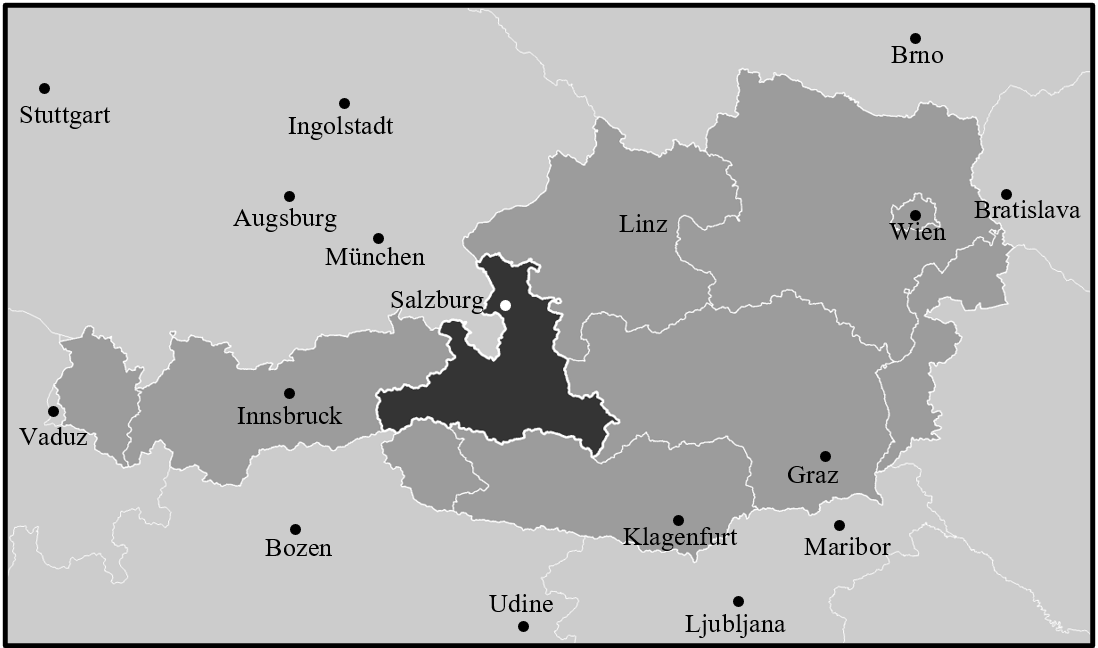
\includegraphics[width=\textwidth]{Figure_1.png}
\caption{\label{fig:blaßnigg:1}Location of Salzburg in Austria (self created image)}
\end{figure}

In addition, parts of Salzburg’s border constitute a national border, stretching over 174\,km, and mostly shared with the Federal Republic of Germany (districts of Berchtesgadener Land and Traunstein), i.e., 164\,km. Only 10\,km in the southwest border on the Tauferer Ahrntal in (German-speaking) South Tyrol (Italy) (cf. \citealt{LandesstatistikSalzburg2022}).

The federal state of Salzburg covers an area of 7,154.6\,km² and has a population of 562,606 inhabitants (01.01.2022).\footnote{For comparison: Austria has a population of approx. 9 million (01.01.2023).} Salzburg consists of six districts, one of which is the city of Salzburg. Perhaps more interestingly from a geolinguistic perspective, Salzburg is also divided into Außergebirg (literally `outside the mountains') in the north and Innergebirg (`in the mountains') in the south of the Northern Limestone Alps (cf. \figref{fig:blaßnigg:2}). This geographical division is accompanied by differences in terms of transport connections and infrastructure and therefore influences the dialectal situation in Salzburg. From a dialectological view, the South-Central Bavarian dialects cover most of Salzburg, a smaller part in the north belongs to the Central Bavarian group. Salzburg is therefore a central space in more than one respect: on the one hand, it is a purely geographical centre, due to the many geopolitical borders involved, and on the other hand, it also constitutes a centre of (dialect) variation, due to its transitional position between different dialect regions.\largerpage[-2]

\begin{figure}
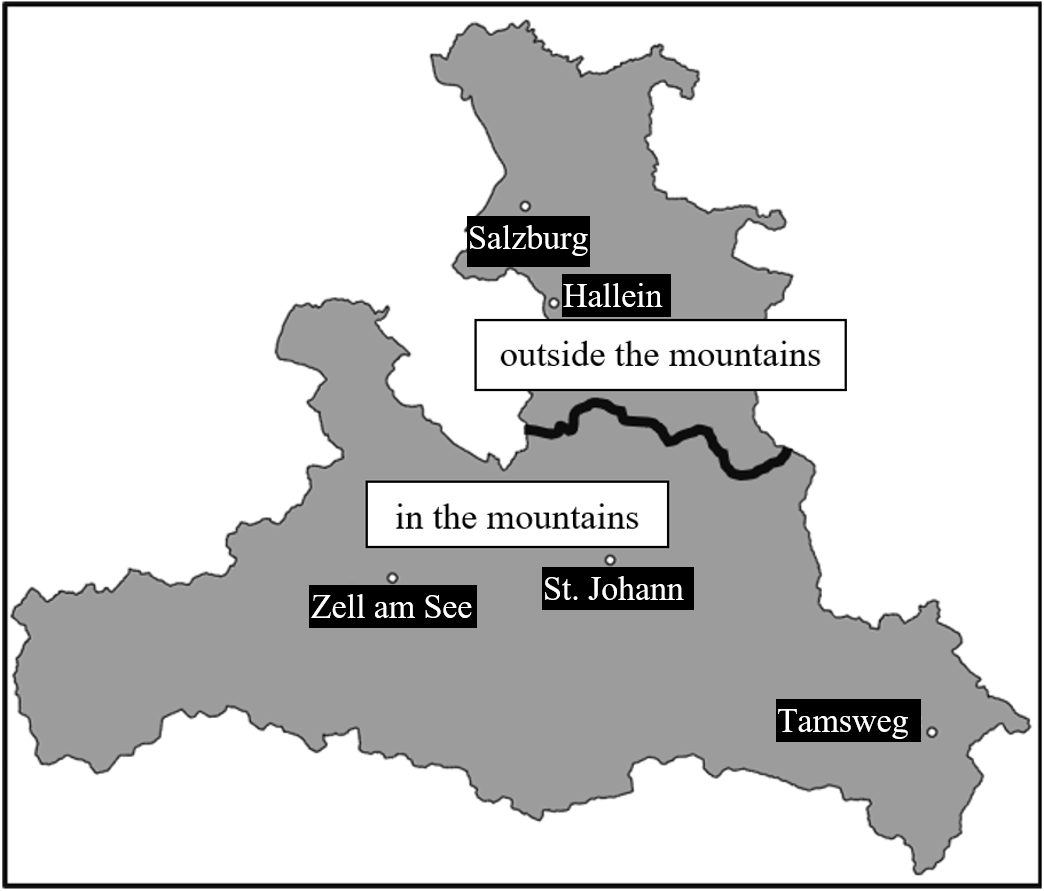
\includegraphics[height=.4\textheight]{Figure_2.png}
\caption{\label{fig:blaßnigg:2}Division between ‘in the mountains’ and ‘outside the mountains’. The border corresponds to the district border between Tennengau and Pongau. N.B.: Populous areas in the South are mostly restricted to valleys. (self-created image)}
\end{figure}

\subsection{State of research and research gaps} \label{sec:blaßnigg:1.3}

Dialectological and variational research has often been conducted only for selected locations in the state of Salzburg. Most studies in Salzburg dialectology (\citealt{Reiffenstein1955, Scheutz2007, Scheutz2022, Scheutzonline, Mauser2021, Mauser2022}) focus exclusively on the base dialect. There are also non-Salzburg-specific research projects which include data from the region like the Task-Cluster B of SFB \textit{Deutsch in Österreich} (DiÖ) ‘German in Austria’, \textit{Wortatlas der deutschen Umgangssprachen} ‘Lexical atlas of colloquial German varieties’ (\citealt{Eichhoff1977, Eichhoff1978, Eichhoff1993, Eichhoff2000}) and \textit{Atlas zur deutschen Alltagssprache} (AdA) ‘Atlas of colloquial German’ (\citealt{ElspaßMöller2003ff}).\footnote{For a popular science publication based on AdA data, cf. \citet{LeemannEtAl2018}.} However, these research projects often only include data on a few locations and usually cannot capture variation within the individual regions of Salzburg.

There are three main aspects which are missing from previous research: first, data that go beyond the local base dialect; second, up-to-date variational data, not least for variation of regiolectal (regional dialect) and near-standard as well as standard lexis; third, more exhaustive and detailed data not restricted to sub-regions or individual locations in Salzburg. Hence, our goal was to conduct a large online survey which draws from the method of the AdA. Its focus on language use includes any point on the vertical variational spectrum in order to grasp colloquial German in Salzburg regardless of its varietal status. In the next section we will elaborate in more detail on what is understood by \textit{colloquial German} and how exactly the data collection took place.

\section{Data and methods} \label{sec:blaßnigg:2}
\subsection{Definition of colloquial language} \label{sec:blaßnigg:2.1}

Dialectological research in Salzburg typically concentrates on the base dialect, often archaic variants produced by NORMs/NORFs (the oldest form possible). The focus of this project, however, is the colloquial German language of the majority of speakers in Salzburg. So what is meant by the term \textit{colloquial German}? 

The project conforms with the AdA’s socio-pragmatic definition of colloquial language:

\begin{quote}
[D]iejenige Sprachform, die in informellen alltäglichen Situationen spontan und routiniert gesprochen wird \citep[419]{Elspaß2010}\footnote{`That form of a language which is spoken spontaneously and routinely in informal everyday situations'.}
\end{quote}

This criterion applies regardless of whether the language used would be categorised linguistically as standard language, regiolect, or (base) dialect. As a consequence, the project targets the whole spectrum of varieties, including the regiolectal and near-standard variants neglected so far.

\subsection{Data collection} \label{sec:blaßnigg:2.2}

For the data collection, the project co-operated with the largest regional newspaper \textit{Salzburger Nachrichten} in order to reach as many speakers as possible. All survey rounds were advertised and published by the \textit{Salzburger Nachrichten}. Items used in the AdA questionnaire were replicated or modified. Some items were adapted to the Salzburg situation, for example in the case of expressions for `female child' several variants in regional dialect were added (round 1, question 2). Additionally, regional variables expected to be more specific to Salzburg were created (e.g. variation of prepositions: \textit{an der Bushaltestelle} vs. \textit{bei der Bushaltestelle} ‘at the bus stop’). Sometimes genuine ASA items were created, i.e., variables that are specifically relevant to the (south-central) Bavarian language area, e.g. subordinate clauses introduced by \textit{dass} versus introduced by \textit{um ... zu} (round 4, question 6) (cf. \citealt{Bayer2020}). The survey participants were asked to select their individual preferred variant from the options given.

Four rounds of questionnaires were distributed from October to December 2019, covering 76 variables of lexis, grammar, phonetics and pragmatics. We also collected multiple types of metadata for a quantitative variational analysis: place of residence, age, gender, highest educational qualification, occupational group, duration of residence and origin of parents. More than 10,000 speakers from Salzburg participated in the survey, of which 9,668 responses have been analysed. Some answers had to be excluded from the analysis due to missing data.

The questionnaire was created using LimeSurvey. We mostly relied on items with single answers but also used multiple answers in some cases, e.g. with variants of greeting and saying farewell. We tried to contextualise the item as much as possible and used visual material to explain meaning and context without additional language input. Each round consisted of approximately 20 thematic items, questions on socio\hyp demographic metadata, and a free-comment section at the end of the questionnaire. The following welcome text provided respondents with an explanatory introduction to the survey:

\begin{quote}
\foreignlanguage{ngerman}{Bitte geben Sie bei den folgenden Fragen an, was man in Ihrem Ort normalerweise hört – egal, ob eher Mundart, eher Hochdeutsch oder etwas dazwischen. Es gibt keine richtigen und falschen Antworten.\\
Am Ende des Fragebogens können Sie (unter „Ihre Anmerkungen“) beschreiben, ob und wie einzelne Ausdrücke unterschiedlich gebraucht werden (z.B. wie häufig, mit welcher unterschiedlichen Bedeutung usw.).\\
Versuchen Sie bitte, sich alle Beispiele in Ihrer ‚normalen’ Aussprache vorzustellen.} (ASA, round 4)\footnote{`In the following questions, please indicate what is normally heard in your location – whether it is more dialect, more High German or something in between. There are no right and wrong answers.\\
At the end of the questionnaire, you can describe (under ``Your comments''), whether and how individual expressions are used differently (e.g. how often, with what different meanings, etc.).\\
Please try to imagine all examples in your “normal” pronunciation.'\\
N.B.: “Hochdeutsch” here is used in its lay meaning “Standard German”.}
\end{quote}

Respondents’ average age (40.7 years) roughly corresponds to that of the federal state (43.1 years). There is a slight overrepresentation of participants with higher educational qualifications (A-levels or degree). However, this is not unusual in surveys originating from the university sector – even if they are disseminated via the regional newspaper (for more details see \citealt[112--114]{NiehausEtAl2022}). Moreover, there are significantly more female than male participants in our survey, the proportion of men is only 33.1\%.

34.4\% of the respondents have always lived in the place for which they provided the information, 18\% for more than 30 years, 37.1\% for more than 10 years, and only 9.2\% have lived there for less than 10 years (no information: 1.3\%). Thus, we can conclude that most respondents are sufficiently familiar with their place of residence and the local language.

\subsection{Data analysis} \label{sec:blaßnigg:2.3}
\subsubsection{Methods used} \label{sec:blaßnigg:2.3.1}

Data was collected and cleaned up, i.e. responses with missing data records were deleted. The remaining total of 9,668 responses from all four rounds were then examined more closely and in detail via SPSS. Statistical analyses were conducted for each district, planning region (see next section) and municipality in Salzburg. At the same time, the metadata were utilised in a quantitative variational analysis, e.g. with regard to gender\footnote{In fact, men and women gave very similar answers to almost all questions. This is the reason why our results are not devalued by the somewhat imbalanced gender ratio.} or age. Furthermore, social factors of regional language use were examined, e.g. whether young women from the city chose significantly more standard (or near-standard) variants than old men from rural areas (who chose variants of traditional dialect more often).

In order to determine whether the results are only due to individual phenomena or indeed similarities across all variables, the data were subjected to a factor analysis with GeoLing as well as a cluster analysis with R. To cluster data we used hierarchical cluster analyses with Ward’s algorithm. For variational linguistic applications, the Ward algorithm seems to be relatively useful as it does not overestimate smaller differences and fluctuations in the data but strongly sanctions larger differences. More information on cluster analysis in general can be found in \sectref{sec:blaßnigg:3.3.1}.

Each item as well as the results of the factor and cluster analyses are finally visualised using ArcGis-Pro, which has proven to be well suited for the cartographic representation of geolinguistic data.

\subsubsection{Basic diatopic levels of analyses} \label{sec:blaßnigg:2.3.2}

Popular belief in Salzburg may refer to several extra-linguistic criteria which index diatopic differences within the federal state. In terms of physical geography, the division into Innergebirg (in the south) and Außergebirg (in the north) is also of some importance. Innergebirg includes the districts of Zell am See (Pinzgau), St. Johann (Pongau) and Tamsweg (Lungau) while the Außergebirg includes the district of Hallein (Tennengau), Salzburg-Land (Flachgau) and the city of Salzburg (cf. \figref{fig:blaßnigg:2}).\footnote{This is reflected, for example, by dialect lexicons compiled by amateurs, which usually attempt to capture the dialect of a district, e.g. \textit{Pinzgauer Mundart Lexikon} \citep{SchwaigerHöck2010}.}

The areas covered by the individual districts differ considerably, for example the largest district in size – the Pinzgau – occupies a cadastral area of 2,641.1\,km² and is thus the third largest district in Austria, whereas the city of Salzburg measures only 65.7~km² and is thus significantly smaller than many municipalities in the federal state (see Figures~\ref{fig:blaßnigg:3} and \ref{fig:blaßnigg:4}). The opposite is true with regard to population size, where the city of Salzburg has the highest number of inhabitants. The data on which the ASA is based was generally analysed at the municipality level. A total of 109 of the 119 municipalities in Salzburg are included in all four rounds of our survey and were thus included in the analyses. Since approx. 92\% of the Salzburg municipalities are represented in all survey rounds, it is possible to conduct fine-grained analyses at the municipal level. At the same time, some municipalities are represented by only a few responses, which means that an analysis of the results in larger areas seems to be useful in order to avoid generating a distorted picture of the actual language use by overrating a few individual answers.

\begin{figure}[p]
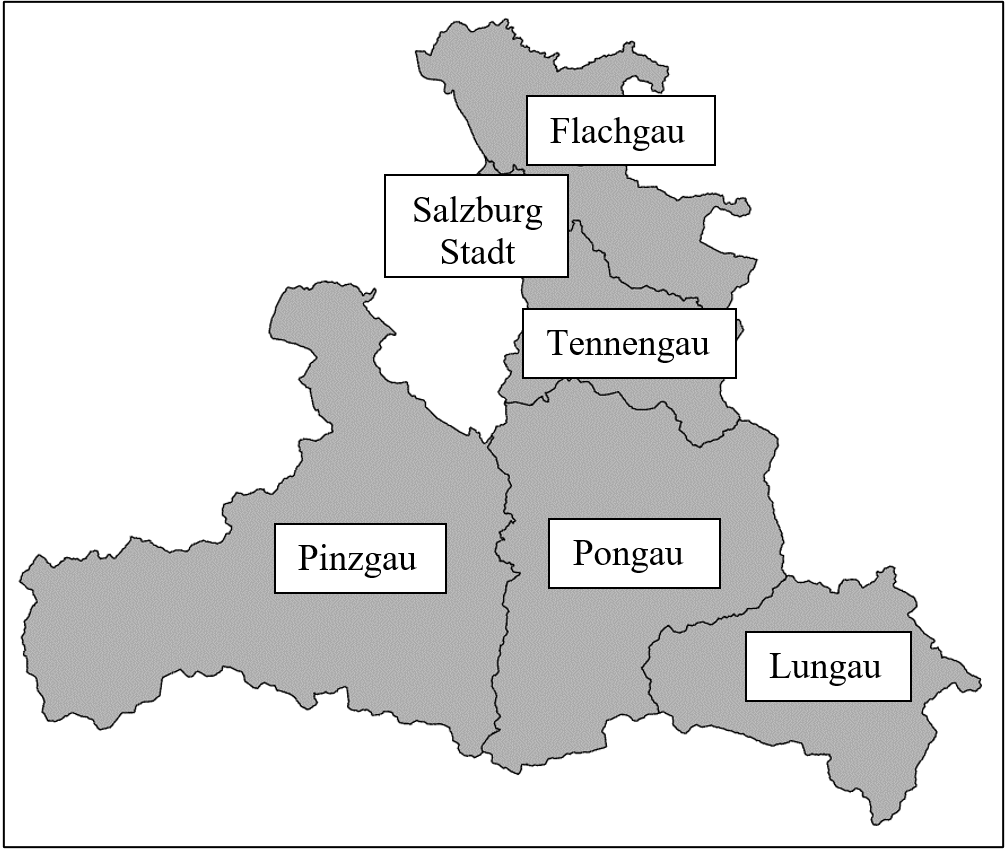
\includegraphics[height=.36\textheight]{Figure_3.png}
\caption{Districts of Salzburg (self created image)}\label{fig:blaßnigg:3}
\end{figure}

\begin{figure}[p]
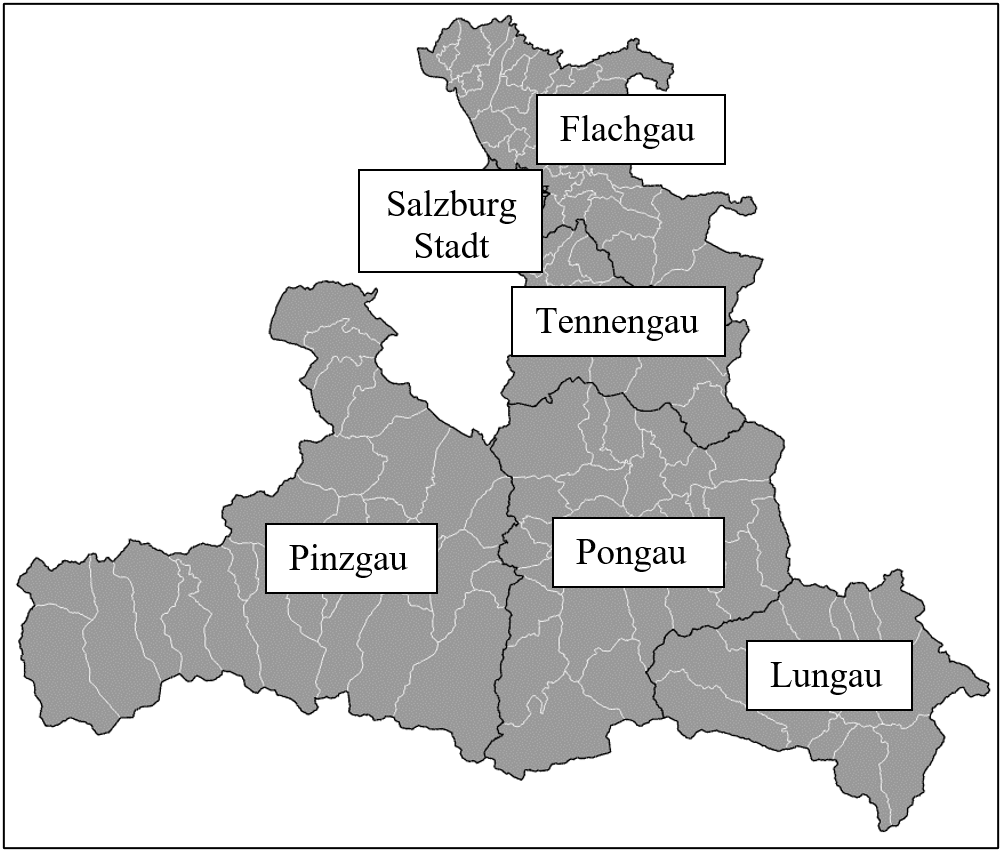
\includegraphics[height=.36\textheight]{Figure_4.png}
\caption{Municipalities in Salzburg (self created image)}\label{fig:blaßnigg:4}
\end{figure}


Districts, on the other hand, often proved too coarse for our variational as well as geolinguistic analyses. For this reason, recourse was made to a level between municipalities and districts: the so-called \textit{planning regions}. The planning regions are a unit of supra\hyp local spatial planning, they are administratively anchored in the national spatial planning programme and also reflect historically-grown regional identities in many cases, which makes them ideal as a basis for geolinguistic analyses in Salzburg. The planning regions offer a good compromise and therefore lie at the core of our quantitative approach and cartography. In an extract from the \textit{Salzburg Regional Development Programme} (revision 2003, published by the Department of Spatial Planning of the Salzburg Federal State Government) the planning regions are defined as follows:

\begin{quote}
\foreignlanguage{ngerman}{Nach dem Raumordnungsgesetz ist es eine der ausdrücklich festgelegten Aufgaben des Landesentwicklungsprogramms, das Land in Planungsregionen zu gliedern. […] Zu Regionen wurden darin nach Anhörung der Gemeinden Gebiete zusammengefasst, die strukturell und funktional zusammengehören und entsprechend den Erfordernissen der Raumordnung als Einheit entwickelt werden sollen, wobei auch die „Identifikation“ der Gemeinden mit einer bestimmten Region berücksichtigt wurde.} \citep[90]{Mair2003}\footnote{`According to the Spatial Planning Act, one of the expressly defined tasks of the Development Programme is to divide the federal state into Regional Spatial Planning Areas [“Planungsregionen”]. [...] After consultation with the municipalities, areas that belong together structurally and functionally and are to be developed as a unit in accordance with the requirements of spatial planning were grouped together in these regions, whereby the ``identification'' of the municipalities with a particular region was also taken into account'.}
\end{quote}

As can be seen, the planning regions are based on national planning as well as regional identities.\largerpage

\begin{figure}
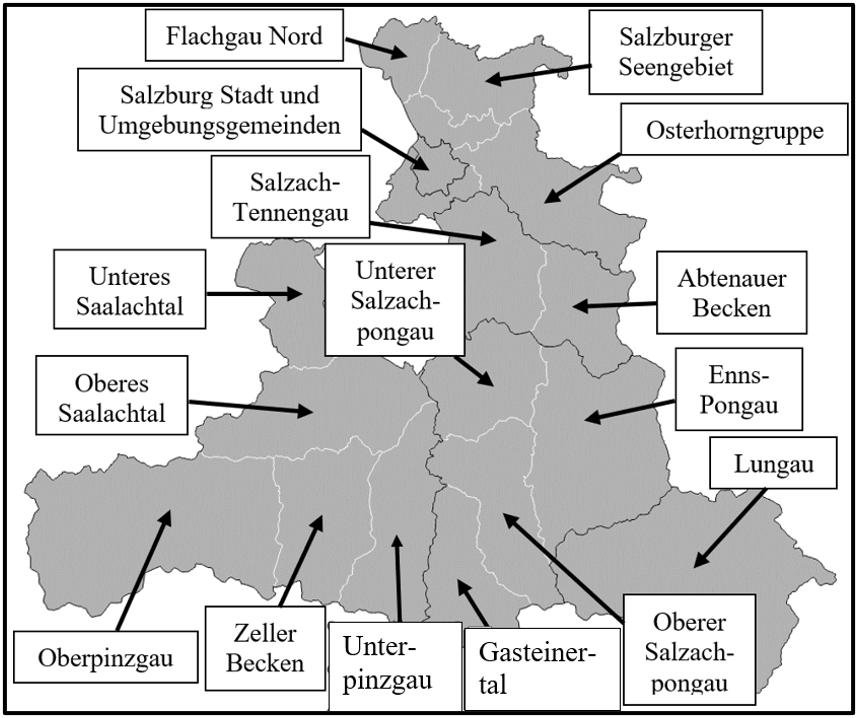
\includegraphics[height=.4\textheight]{Figure_5.png} \label{fig:blaßnigg:5}
\caption{Official regional planning regions (cf. \citealt{Mair2003}) -- (self created image)}
\end{figure}

Each of the 16 planning regions in the province of Salzburg consists of an average of seven municipalities. As far as the number of respondents per planning region is concerned, numbers range from 102 (round 4, Zeller Becken) to 1003 (round 1, Lungau) per 100,000 inhabitants. These numbers ensure a realistic approximation to inner-regional language use in Salzburg while at the same time much more detailed insights can be gained than if only the district level were considered. Additionally, analyses were carried out at district and municipality level in order to avoid pitfalls during interpretation; most importantly, we applied multidimensional scaling (MDS) on both levels, which allows for a calculation of linguistic similarities.

\section{Findings} \label{sec:blaßnigg:3}
\subsection{Mapping: General approach} \label{sec:blaßnigg:3.1}

The following maps depict one variable each, i.e. dominant variants in a combined heat map. For this purpose, each dominant variant is given its own colour, while the relative frequency of the dominant variant is represented by colour intensity. Put simply: the more intense the colour, the stronger the prevalence of a variant. All sub-divisions on the maps are based on the planning regions, with district boundaries and the respective district capitals visualised for better orientation. At the same time, many maps show that the distribution of individual phenomena is often not identical with district boundaries, which increases the additional informative value of analyses at the level of planning regions. To illustrate this, two maps will be showcased below and their results will be presented as examples. The presented maps (Figures~\ref{fig:blaßnigg:6} and \ref{fig:blaßnigg:7}, page~\pageref{fig:blaßnigg:6}) should be understood such that the intensity of the color~-- either red or blue~-- correlates with the prevalence of the variant. The stronger the color shading, the more widespread the variant.

\begin{figure}[p]
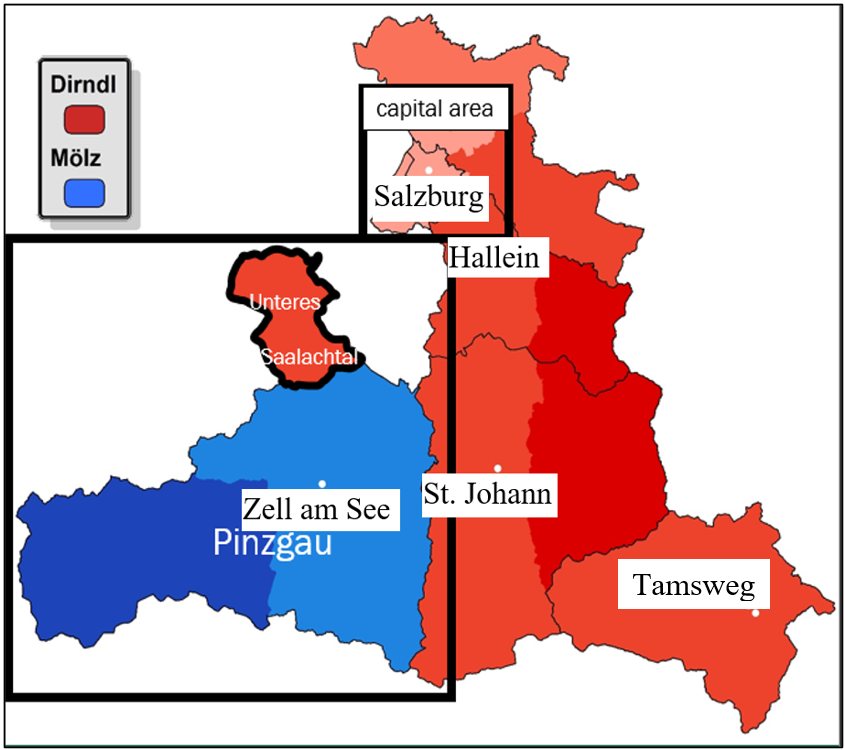
\includegraphics[height=.4\textheight]{Figure_6.png}
\caption{Names for `female child' (self created image)} \label{fig:blaßnigg:6}
\end{figure}

  
\begin{figure}[p]
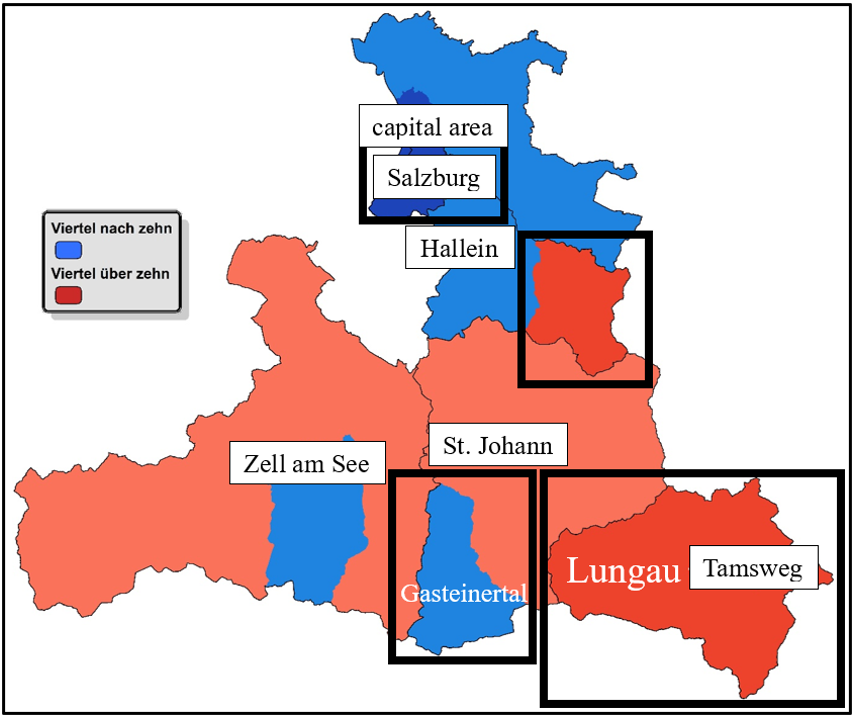
\includegraphics[height=.4\textheight]{Figure_7.png}
\caption{Verbalisation of \textit{10:15} (self created image)} \label{fig:blaßnigg:7}
\end{figure}

\subsection{Showcase results} \label{sec:blaßnigg:3.2}
\subsubsection{Example `female child'} \label{sec:blaßnigg:3.2.1}

The designations for `female child' are a classic in German{\hyp}speaking dialectology. The German dialects in general, including those spoken in Austria, boast a multitude of expressions and phonetic variants of these expressions for referring to the category of `female child'. Our results for Salzburg show that two expressions are particularly common here: \textit{Mölz} and \textit{Dirndl}.

The south-western region of the Pinzgau is strongly dominated by \textit{Mölz} except for the Unteres Saalachtal (‘Lower Saalach Valley’), an area in the northern Pinzgau. This demonstrates the strength of working with planning regions, for the popular assumption that \textit{Mölz} is the preferred term for `female child' in the entire Pinzgau cannot be confirmed by our data. Our survey would also have yielded this very result if the districts alone had been the basis of our cartographic representation. By using planning regions, however, it becomes apparent on the one hand, that there is a region in the Pinzgau where \textit{Mölz} is not at all the dominant variant and, moreover, that the frequency of this particular variant differs within the district, specifically that \textit{Mölz} is used most frequently in the far west. Similar observations can be made for \textit{Dirndl}: Although it is the most frequently used variant throughout the rest of the federal state, usage is particularly frequent in the east of the federal state. In the capital area around the city of Salzburg, \textit{Dirndl} is only just the most frequently mentioned designation for `female child': Although it is still dominant, there is a higher percentage of standard variants – and more variation in general (which does not come as a surprise and applies to many variables). In addition to \textit{Dirndl}, the standard German \textit{Mädchen} (approx. 17\%) and near-standard \textit{Mädl} (approx. 36\%) are also frequently used in and around the city of Salzburg. Hence, \textit{Dirndl} is not a quasi-absolute default variant in most of the federal state but a relatively dominant variant most prevalent in the east.

\subsubsection{Example \textit{10:15}} \label{sec:blaßnigg:3.2.2}
A particularly suitable item for our demonstration of the data is the verbalisation of a certain time of day, in (standard) English \textit{ten-fifteen} or \textit{quarter past ten}. To avoid verbal stimuli, this question only showed a picture of a clock and asked for the phrase to name the corresponding time. The German variants in the state of Salzburg are \textit{Viertel nach zehn} `quarter past ten' (in blue) and \textit{Viertel über zehn} `quarter over ten' (in red). The map (\figref{fig:blaßnigg:7}) demonstrates a pattern which surfaces often in our data, i.e. an opposition between the more urban north (capital area) and the more rural southeast (Lungau), notwithstanding a few exceptions such as the northern Abtenauer Becken (`Abtenau basin'), which often joins the language use of the south – and vice versa the southern Gasteinertal (`Gastein valley'), which often conforms with the language use of the northern capital area. Within the individual districts clear-cut areas with different degrees of variant use become apparent.

\subsection{Results of cluster analyses} \label{sec:blaßnigg:3.3}
\subsubsection{General approach} \label{sec:blaßnigg:3.3.1}

Our data have a nominal scale form (as is customary in variational linguistics) and can easily be spread in a table: Each row of the table contains the data of exactly one informant. The columns represent the variables of the survey, the individual cells contain the respective variant that the informant has given for the variable. As already mentioned, most of the variables are of a purely linguistic nature, with the exception of the metadata information on the respondents as well as the free comments section. These are also documented individually for each informant.

This was the basis on which we evaluated the most prevalent variants for each planning region. However, our interest is not only in the results for each individual item but we also wanted to identify inter-local and inter-regional similarities, which only become apparent with a sufficient amount of  data combined. Factor and cluster analyses are suitable for such approaches (cf. \citealt[509]{Goebl2005}, \citealt[234--235]{PröllEtAl2021}, note  14). In the following, the results of the cluster analysis will be presented.

The basis for these further analytical steps is no longer the original table of nominally scaled, individual raw data, but a table with the relative frequencies of the individual variants per survey location. These calculations were conducted for all our diatopic levels of analysis, i.e. the districts, the planning regions, and single municipalities. In the present paper, we will only take a closer look at two cluster maps which are based on the planning regions. A distance matrix of the planning regions to each other is calculated from the relative frequencies of the linguistic variants per planning region. In order to make this high-dimensional variation less complex and interpretable, cluster analysis was used: The individual planning regions were grouped based on their similarity or dissimilarity. These groups (= clusters) should be as homogeneous as possible within themselves and at the same time as different as possible from each other. Ultimately, therefore, one obtains a concrete allocation of the individual regions to groups, which in turn can be represented and interpreted cartographically. These groupings can be represented at different levels of granularity, e.g. as a 2-cluster, 3-cluster or 4-cluster solution. 

\begin{figure}
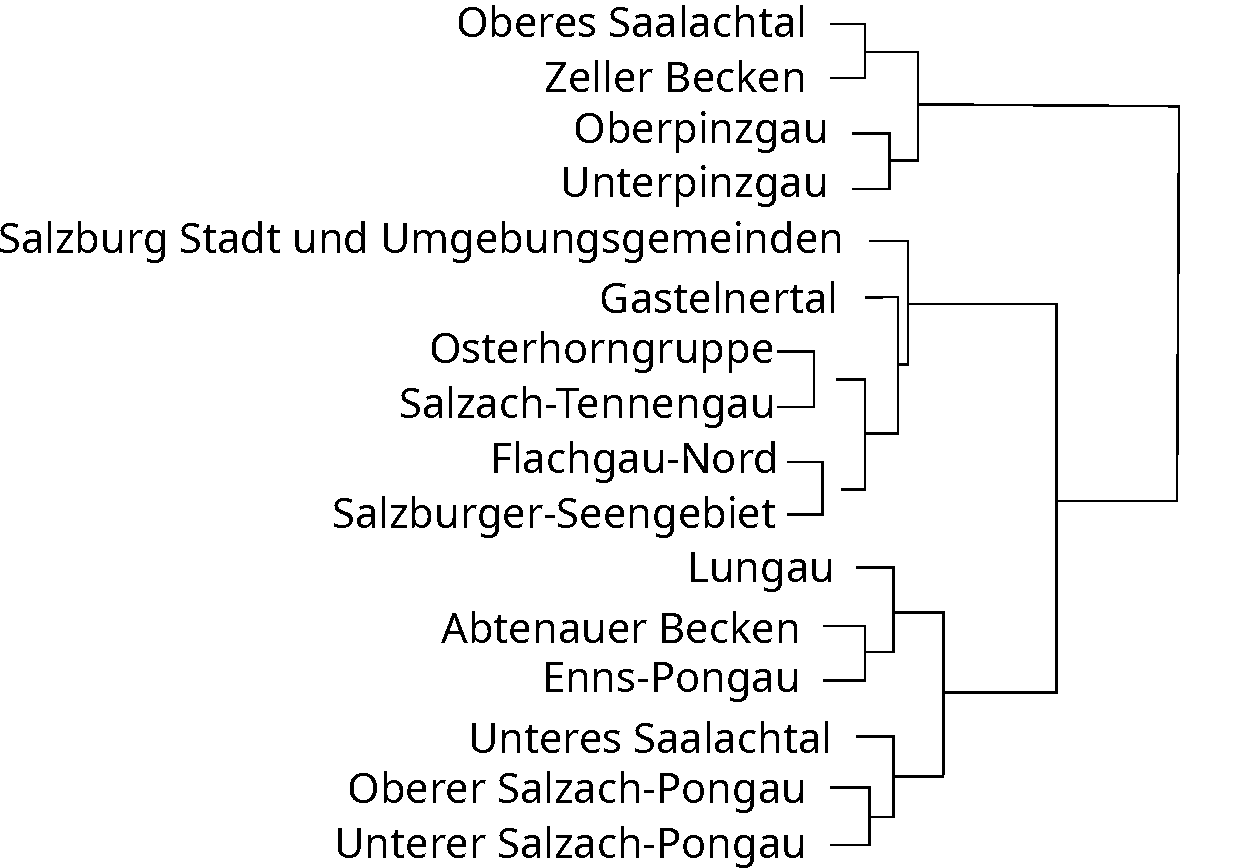
\includegraphics[height=.4\textheight]{blaßnigg-img008.pdf}
\caption{Cluster analysis dendrogram (self created image)}
\label{fig:blaßnigg:8}
\end{figure}

The allocation of the planning regions to individual clusters is best represented in the form of a dendrogram (cf. \figref{fig:blaßnigg:8}). Depending on where the cut is made to distinguish clusters, solutions with different numbers of clusters are obtained. Since the length of the horizontal lines provides information about the linguistic distance between the individual clusters, the dendrogram can also be used to determine which cluster solutions ultimately represent plausible groupings.

As can be seen from the dendrogram, mainly 2-, 3- and 4-cluster solutions are suitable. We will briefly discuss a 3- and a 4-cluster solution.

\subsubsection{3-cluster solution} \label{sec:blaßnigg:3.3.2}

Popular belief as to how the federal state of Salzburg could be divided into dialect areas include the idea that there is a clear linguistic division between the dialects Außergebirg (`outside the mountains', i.e. in the north) and Innergebirg (`in the mountains', i.e. in the south). In addition, political districts are ascribed their own regional dialects such as \textit{Pinzgauerisch} in the south-western part of the state and the like. The 3-cluster map (cf. \figref{fig:blaßnigg:9}) shows that the actual linguistic situation is clearly more complex.

  
\begin{figure}
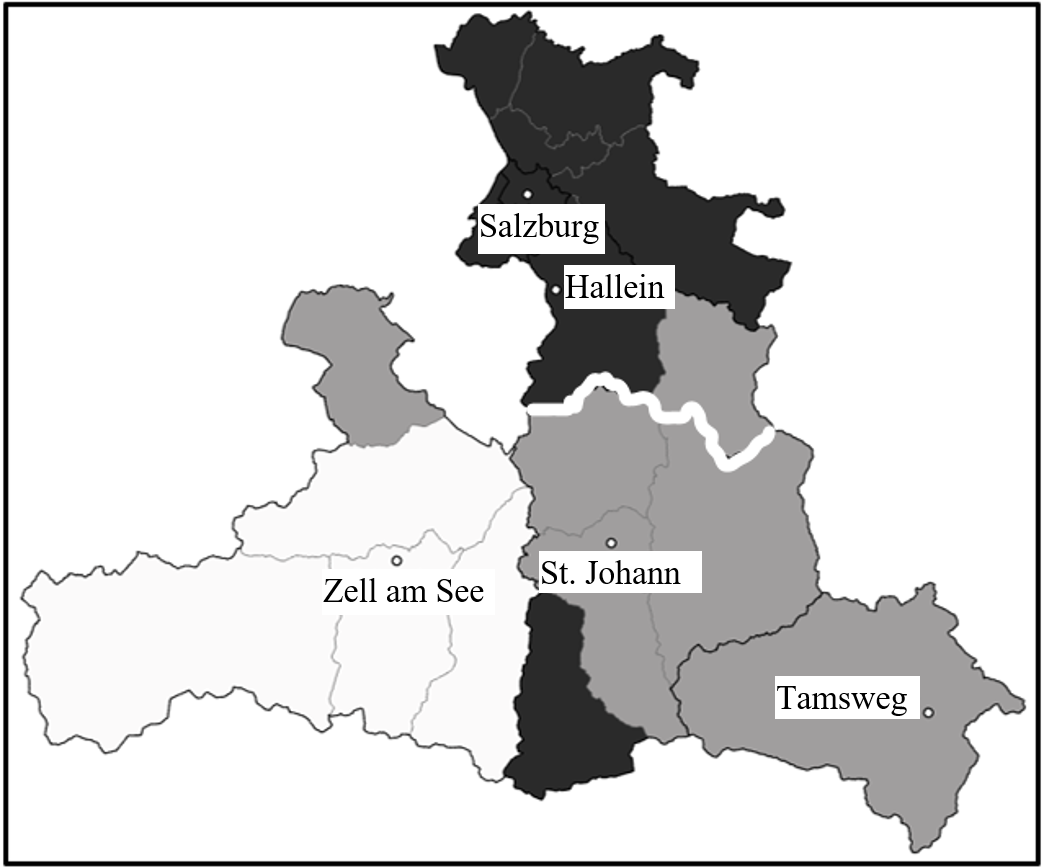
\includegraphics[height=.4\textheight]{Figure_9.png}
\caption{3-cluster solution (self created image)}
\label{fig:blaßnigg:9}
\end{figure}

In addition to the boundaries of the planning regions and the district capitals, we also drew the border between Innergebirg and Außergebirg (bold white line). The border runs between the two districts of Tennengau and Pongau. From the perspective of physical geography, the lay-linguistic notion is understandable: Some Salzburgers from the Innergebirg travelling to the capital will immediately notice a change, when the Salzach valley widens outside the Pass Lueg and the rugged mountains give way to gentle hills, and, of course, natural obstacles can be a factor of linguistic variation. However, linguistic difference may subjectively be perceived as much more salient and relevant than the distance measured by linguistic means. For example, the Abtenauer Becken (in grey, north of the white line – a basin in terms of geology) clearly belongs to the south in terms of linguistic distance in this cluster solution. On the other hand, the cluster resembling the Außergebirg area (black) also includes the Gasteinertal in the south, which is geographically clearly a mountain valley of the south. On top of that, the Innergebirg does not add up to a single cluster but instead consists of three clusters, mainly two large clusters in white and in grey in the (south-)west and in the (south\nobreakdash-)east respectively. Not even the Pinzgau district (white) consists of a single cluster, as again the northern part, Unteres Saalachtal, belongs to a different cluster – a phenomenon which could already be observed with the lexical variants of `female child' (see \sectref{sec:blaßnigg:3.2.1}, \figref{fig:blaßnigg:6}). The map for `10:15' (see \sectref{sec:blaßnigg:3.2.2}, \figref{fig:blaßnigg:7}) again shows very well the outliers also evident in the 3-cluster solution, namely the Abtenauer Becken and the Gasteinertal, which in many maps stand out with regard to other linguistic variables from their surroundings. In sum, it can be said that neither the linguistic relevance of political districts nor the popular binary distinction of varieties \textit{in} and \textit{outside} the mountains can be confirmed through our cluster analysis. Rather, it seems that other factors play a crucial role, such as the infrastructural proximity to the city of Salzburg. At the same time, the cluster which mainly covers the south-east and centre-most areas seems to form a transition area between the urban north around the city of Salzburg and the rural south(-west). The fact that regional centres such as St. Johann im Pongau are relatively well-connected to the city of Salzburg in terms of infrastructure seems to be at work here. Even from the Unteres Saalachtal – via a short route through German territory – you can reach the city of Salzburg relatively fast, from some places (e.g. Unken) even faster than the district’s own capital, Zell am See.

\subsubsection{4-cluster solution} \label{sec:blaßnigg:3.3.3}

The 4-cluster solution (see \figref{fig:blaßnigg:10}) can refine the 3-cluster picture a little more: Differences to the 3-cluster solution are especially evident in the transition area, which now breaks up into two clusters.

  
\begin{figure}
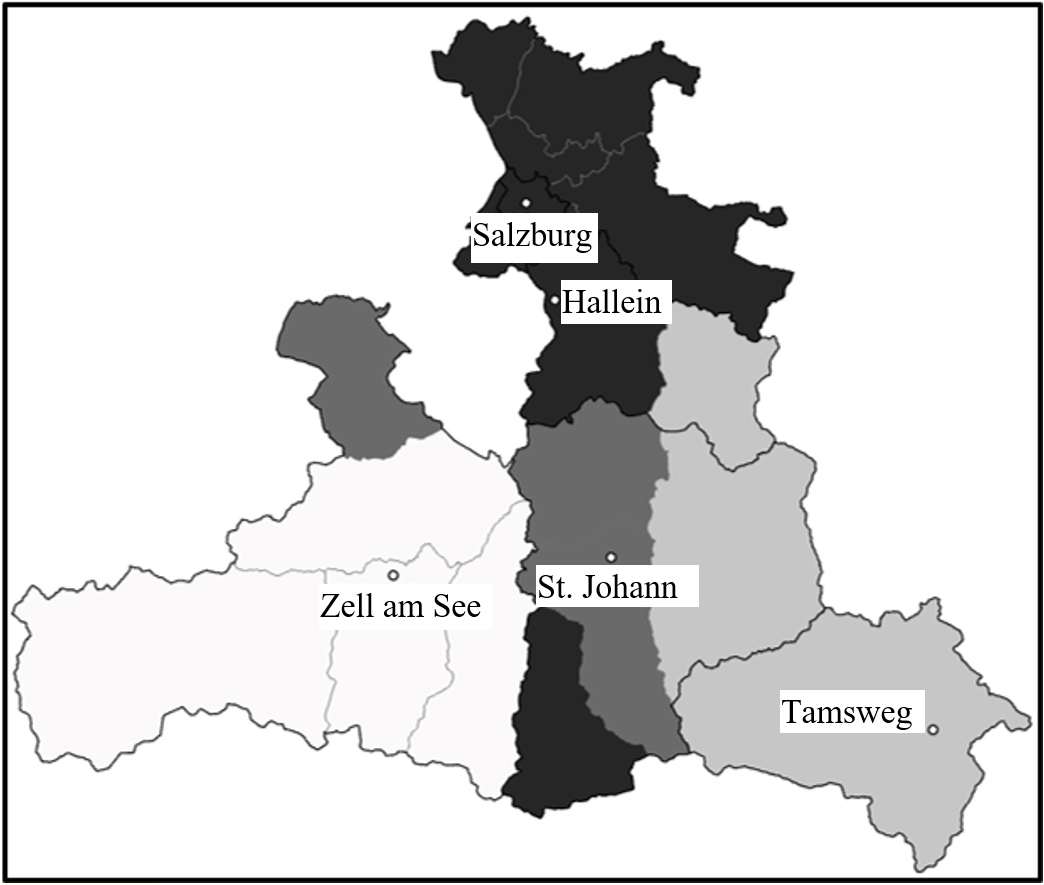
\includegraphics[height=.4\textheight]{Figure_10.png}
\caption{\label{fig:blaßnigg:10} 4-cluster solution (self created image)}
\end{figure}

Similar to the 3-cluster solution, there is a pseudo-Außergebirg cluster (in black), with a tendency towards either standard variants or Bavaro-Austrian regiolectal variants (that is, variants which are also common in other parts of Austria and in south-eastern Germany/Bavaria). In the Innergebirg, the large eastern cluster of the 3-cluster solution breaks apart into smaller clusters, one transition area more similar to the northern cluster (in dark grey) and the easternmost rural area, which maintains base dialect variants more strongly (in light grey).
\largerpage

The differences between the dark grey and the light grey clusters can be illustrated by numerous examples: the Pongau central area (in the west of the district of St. Johann in dark grey) more often tends to use variants that are common in the city of Salzburg and its surroundings, e.g. the grammatical gender of email, neutr. \textit{das} \textit{E-Mail} (Enns-Pongau) vs. fem. \textit{die} \textit{E-Mail} (Pongau central area). The West (in white) is obviously orientated towards dialect variants similar to those of adjacent west Austrian dialects, such as Tyrolean, a relatively stable result regardless of the number of clusters.\footnote{Cf. data in the \textit{Tiroler Dialektarchiv} (Archive of Tyrolean Dialects): \url{https://www.tiroler-dialektarchiv.at}. For instance, \textit{Mölz} appears as \textit{Mötz} in Tyrol, cf. \url{https://wiki.uibk.ac.at/tda/index.php/Bedeutung_14}.}

The assumption that the infrastructural proximity to the city could play a decisive role is corroborated by this 4-cluster solution. Those regions of the original transition cluster in the 3-cluster solution which are particularly well connected to the city of Salzburg now fall into the more urban, regiolectal\footnote{Common standard linguistic variants would be, for example, \textit{Mädchen} ‘female child’ as opposed to regiolectal \textit{Dirndl} and dialectal \textit{Mölz/Tåttn}, but also pronunciation variants such as [{}'mɪlç] \textit{Milch} ‘milk’ as opposed to regiolectal [{}'myːç] and dialectal [{}'miːç] as well as subjunctive II constructions such as (\textit{wir}) \textit{bräuchten} ‘we would need’ as opposed to regiolectal \textit{täten}/\textit{dadn ... brauchen} and dialectal \textit{brauchatn} (cf. also \citealt{NiehausEtAl2022}).} transition cluster (dark grey), while the eastern and southeastern regions (light grey) are closer to the rural-dialectal forms of the southwest (white). This interpretation is corroborated by an MDS-analysis.
\largerpage[2]

Once again, however, the Gasteinertal in the south (black), which is located \textit{in} the mountains, joins the northern urban cluster. Infrastructural proximity to the city can hardly account for this. Yet, a long-standing history of (health and spa) tourism and subsequent migration (e.g. German or Viennese retirement residences in the Gasteinertal, going back as far as the late 19th century) may explain the similarities of the Gasteinertal and the northern regions: It entails either the tendency to converge towards wider regional, non-local variants or to use standard variants. Historical migration through jobs in tourism and retirement could have left a linguistically sustainable mark by changing the composition of the population. We will pursue this case further in the future, among other factors that still await analysis. 

\section{Conclusion and outlook} \label{sec:blaßnigg:4}

In addition to traditional dialect areas and popular divisions (Innergebirg/Außer\-gebirg), which are only partially confirmed by our data, various factors influence patterns of language variation in the federal state of Salzburg.

Our analysis has demonstrated that infrastructural proximity to the city of Salzburg seems to be a major factor which may have contributed to creating a transitional regiolect. Infrastructure seems to be at least as important as mere geographical distance, sometimes it even trumps the latter. In other cases, this results in groups of diatopic variants which can only be explained by consulting both factors: The Abtenauer Becken, for example, is geographically closer to the city of Salzburg than, for example, St. Johann. However, St. Johann is better connected to the city of Salzburg in terms of infrastructure due to the nearby motorway and the railway connection. The MDS-analysis mentioned above shows that St. Johann is in fact linguistically closer to the city of Salzburg than the Abtenauer Becken.

Smaller regional centers also play a certain role in many cases (in addition to the city of Salzburg as the overall centre of the federal state). These are often also the target of commuter flows and usually have a better infrastructure than many rural communities in the mountain regions. At the same time, these regional centres often show linguistic characteristics that bring them closer to the regiolectally influenced urban language of the capital than to the rural base dialects which surround these regional centres. In sum, the situation is strongly reminiscent if not a prime example of \citegen{Trudgill1974} gravity model where linguistic change spreads from one (urban) centre to another and only then diffuses into the surrounding areas. Accordingly, there appears to be a preservation of traditional dialect variants outside these smaller centres, i.e. in the westernmost and easternmost rural parts of Salzburg, in contrast to more dynamic areas in the north.
\largerpage[2]

This insight has been gained by a combination of quantitative analyses which are sufficiently fine-grained and could be complemented by qualitative studies to account for the data in future approaches. As the case of the Gasteinertal has shown, even with comprehensive statistics for a large amount of data one must take into account the specific histories of locations which can leave their mark linguistically, irrespective of geographic and/or infrastructural circumstances. 

Finally, social factors such as age  and profession are expected to play a significant role for the regional language use in Salzburg (e.g. young urban vs. old rural). Analyses on these factors will be presented in forthcoming research.

\sloppy\printbibliography[heading=subbibliography,notkeyword=this]
\end{document} 
